\section{Introduction}
The easiest way to implement a dynamic language such as Python is to write an
interpreter; however, interpreters are slow.

The alternative is to write a compiler; writing a compiler that targets a high
level virtual machine like CLI or JVM is easier than targeting a real CPU, but
it still requires a lot of work, as IronPython, Jython, JRuby demonstrate.

Moreover, writing a static compiler is often not enough to get high
performance; IronPython and JRuby are going in the direction of JIT compiling
specialized versions of the code depending on the actual values/types seen at
runtime; this approach seems to work, but writing it manually requires an
enormous effort.

PyPy's approach \cite{RiBo07_223} is to automatize the generation of JIT compilers in order
to minimize the effort required to get a fast implementation of a
dynamic language; automatic generation of JIT compilers is done with
the help of partial evaluation techniques and requires the user only
to provide an interpreter with some manual annotations which hint
the generator how interpretation and JIT compilation has to be interleaved. 

More precisely, in this paper we focus on the ability of generating a JIT compiler able to emit code
for the .NET virtual machine. To our knowledge, this is the first experiment with an interpreter with
two \emph{layers} of JIT compilation, since, before being executed, the
emitted code is eventually compiled again by .NET's own JIT compiler.

The contributions of this paper are twofold: (1) \emph{promotion} is a
generalization of polymorphic inline caches that make partial evaluation
practical for dynamic languages; (2) we demonstrated that the idea of
\emph{JIT layering} can give good results, as dynamic languages can be even
faster than their static counterparts.

\subsection{PyPy and RPython}

\commentout{
\begin{figure}[h]
\begin{center}
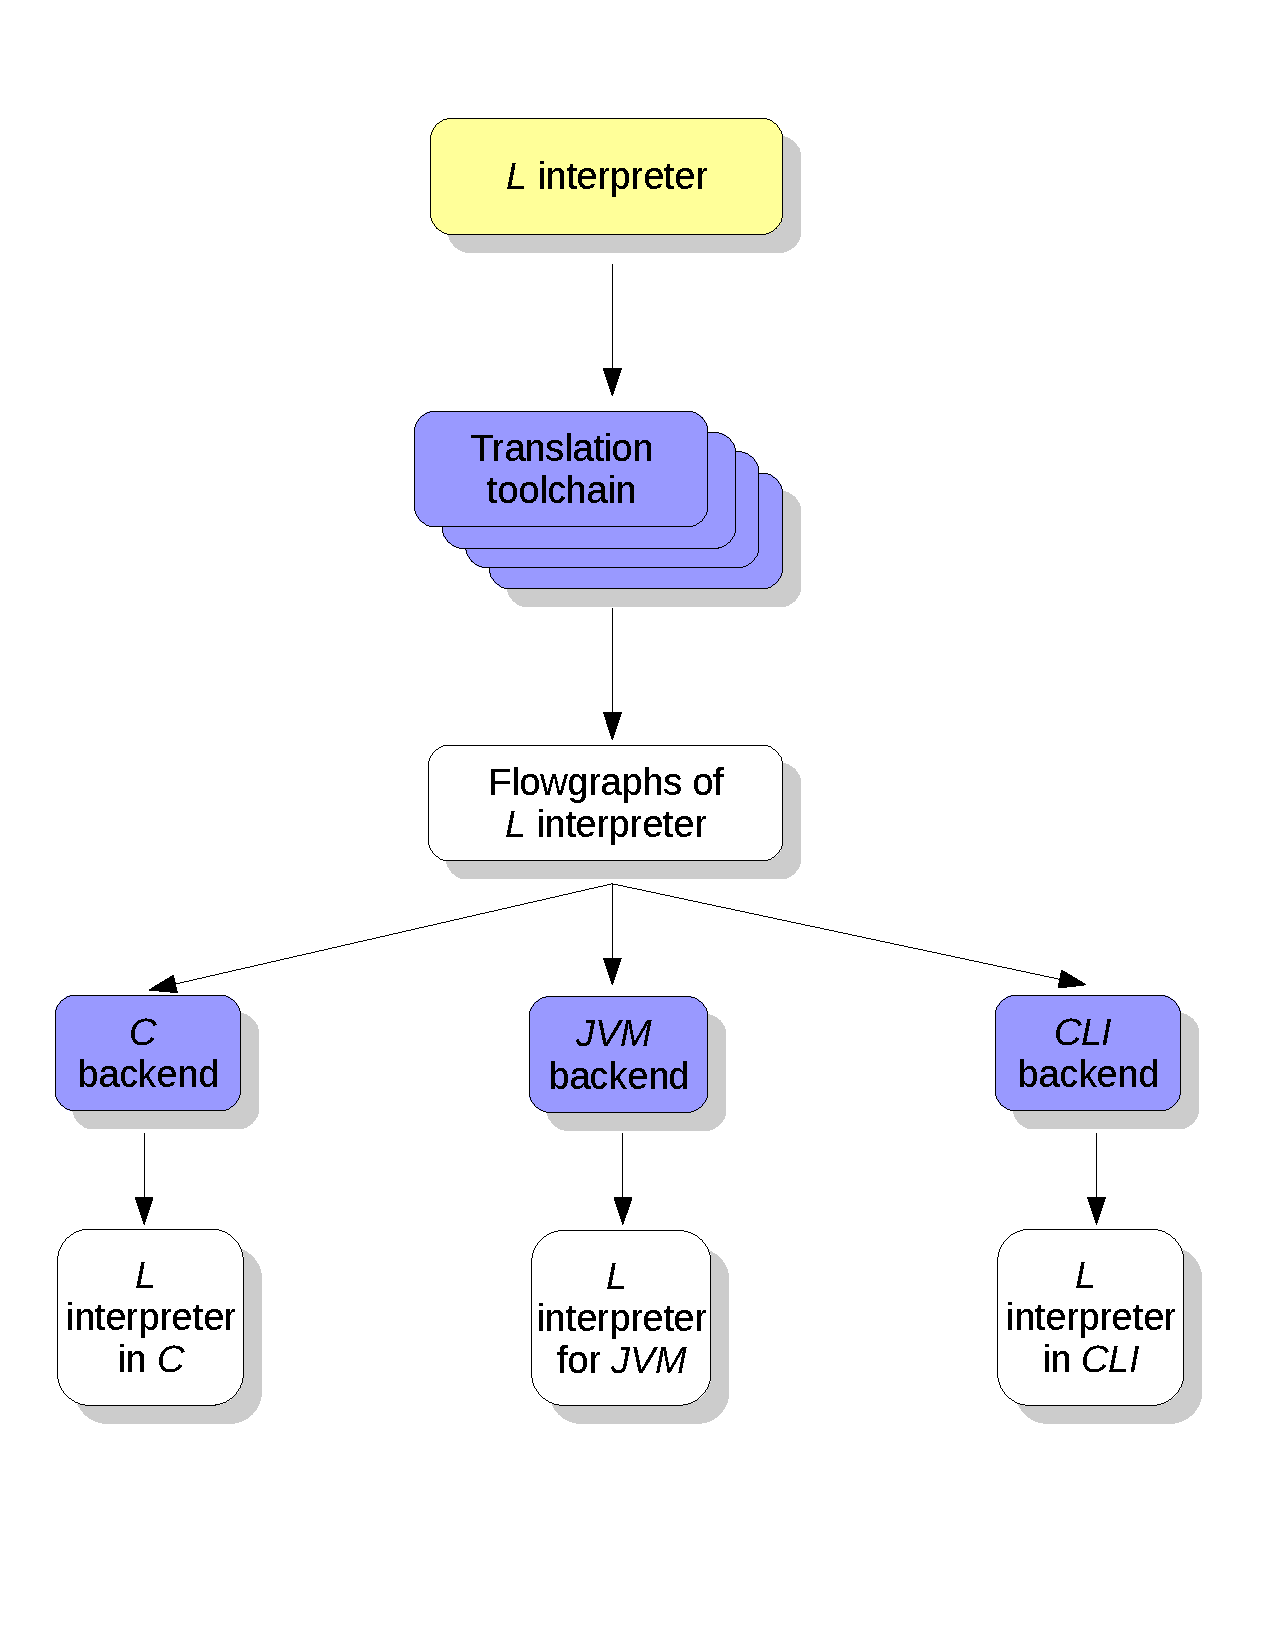
\includegraphics[width=.6\textwidth]{diagram0}
\caption{PyPy infrastracture for generating an interpreter of a
  language $L$ for several platforms}\label{pypy-fig}
\end{center}
\end{figure}
}

The \emph{PyPy} project\footnote{\texttt{http://codespeak.net/pypy/}}
\cite{RigoPedroni06} was initially conceived to develop an implementation of Python which
could be easily portable and extensible without renouncing efficiency.
To achieve these aims, the PyPy implementation is based on a highly
modular design which allows high-level aspects
to be separated from lower-level implementation details.
The abstract semantics of Python is defined by an interpreter written
in a high-level language, called RPython \cite{AACM-DLS07}, which is in fact a subset of
Python where some dynamic features have been sacrificed to allow an
efficient translation of the interpreter to low-level code.

Compilation of the interpreter is implemented as a stepwise
refinement by means of a translation toolchain which performs type
analysis, code optimizations and several transformations aiming at 
incrementally providing implementation details such as memory management or the threading model.
The different kinds of intermediate codes  which are refined 
during the translation process are all represented by a collection of control flow graphs,
at several levels of abstractions.

Finally, the low-level control flow-graphs produced by the toolchain
can be translated to executable code for a specific platform by a
corresponding backend.
Currently, three fully developed backends are available to produce
executable C/POSIX code, Java and CLI/.NET bytecode. 

Despite having been specifically developed for Python, the PyPy infrastructure
can in fact be used for implementing other languages. Indeed, there were
successful experiments of using PyPy to implement several other languages such
as Smalltalk \cite{BolzEtAl08}, JavaScript, Scheme and Prolog.

\commentout{
As suggested by Figure~\ref{pypy-fig}, a portable interpreter for a
generic language $L$  can be
easily developed once an interpreter for $L$ has been implemented in
RPython.
}

\subsection{PyPy and JIT-Generation}

One of the most important aspects that PyPy's translation toolchain can weave
in is the \emph{automatic generation of a JIT compiler}.  This section will
give a high-level overview of how the JIT-generation process works. More
details will be given in subsequent sections.

The first step is to write an interpreter for the chosen language.  Since it
must be fed to the translation toolchain, the interpreter has to be written in
RPython.  Then, to guide the process, we need to add few manual
annotations to the interpreter, in order to teach the JIT generator which
informations are important to know at compile-time.  Annotations are inserted
as \emph{hints}, as described in section \ref{sec:hints}.

It is important to distinguish between three distinct phases of execution:

\begin{enumerate}
\item \textbf{Translation-time}: when the translation toolchain runs and the
  JIT compiler is automatically generated from the interpreter.  The result is
  an executable that can be used to run programs written in the chosen
  language.
\item \textbf{Compile-time}: when the JIT compiler runs, generating executable
  code on the fly.
\item \textbf{Runtime}: when the code generated at compile-time is executed.
\end{enumerate}

Note that in this schema translation-time happens only once, on the
developer's machine.  By contrast, compile-time and runtime happens every time
the user wants to run some program.

Generating efficient compilers for dynamic languages is hard.  Since these
languages are dynamically typed, usually the compiler does not have enough
information to produce efficient code, but instead it has to insert a lot of
runtime checks to select the appropriate implementation for each operation.

By emitting code at runtime, JIT compilers can exploit some extra knowledge
compared to traditional static compilers.  However, we need to take special
care to choose a strategy for JIT compilation that lets the compiler to take
the best of this advantage.

Most JIT compilers for dynamic languages around (such as
IronPython\footnote{http://www.codeplex.com/IronPython},
Jython\footnote{http://www.jython.org/} or
JRuby\footnote{http://jruby.codehaus.org/}) compile code at the method
granularity.  If on the one hand they can exploit some of the knowledge
gathered at runtime (e.g. the types of method parameters), on the other hand
they can do little to optimize most of the operations inside, because few
assumptions can be made about the global state of the program.

JIT compilers generated by PyPy solve this problem by delaying the compilation
until they know all the informations needed to generate efficient code.  If at
some point the JIT compiler does not know about something it needs, it
generates a callback into itself and stops execution.  

Later, when the generated code is executed, the callback might be hit and the JIT
compiler is restarted again.  At this point, the JIT knows exactly the state
of the program and can exploit all this extra knowledge to generate highly
efficient code.  Finally, the old code is patched and linked to the newly
generated code, so that the next time the JIT compiler will not be invoked
again.  As a result, \textbf{runtime and compile-time are continuously
interleaved}. The primitive to do this sort of interleaving is called promotion,
it is described in Section \ref{sec:promotion}.

One of the most important optimizations that the generated JIT does is removing
unnecessary allocations. This is described in Section \ref{sec:virtuals}

Modifying the old code to link to the newly generated one is very challenging on
.NET, as the framework does not offer any primitive to do this.  Section
\ref{sec:clibackend} explains how it is possible to simulate this behaviour.
